\section{Durchführung}
\label{sec:Durchführung}

\subsection{Versuchsaufbau}
\label{sec:Versuchsaufbau}
%\begin{figure}
%	\centering
%	\caption{Schematische Darstellung des Versuchsaufbaus \cite{anleitung}.}
%	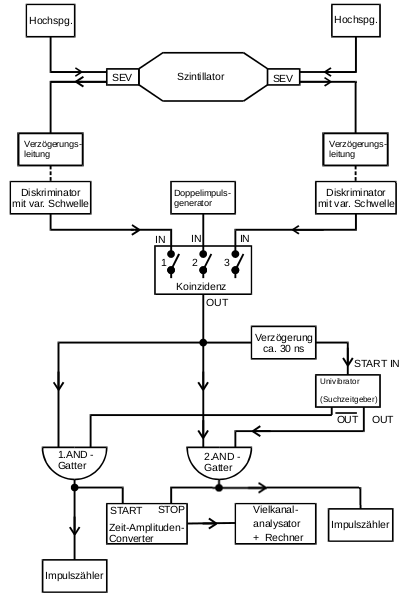
\includegraphics{Bilder/aufbau.png}
%	\label{fig:aufbau}
%\end{figure}
%
%\begin{figure}
%	\centering
%	\caption{Schematische Darstellung der Quelle zur Erzeugung radioaktiven Isotopen \cite{anleitung}.}
%	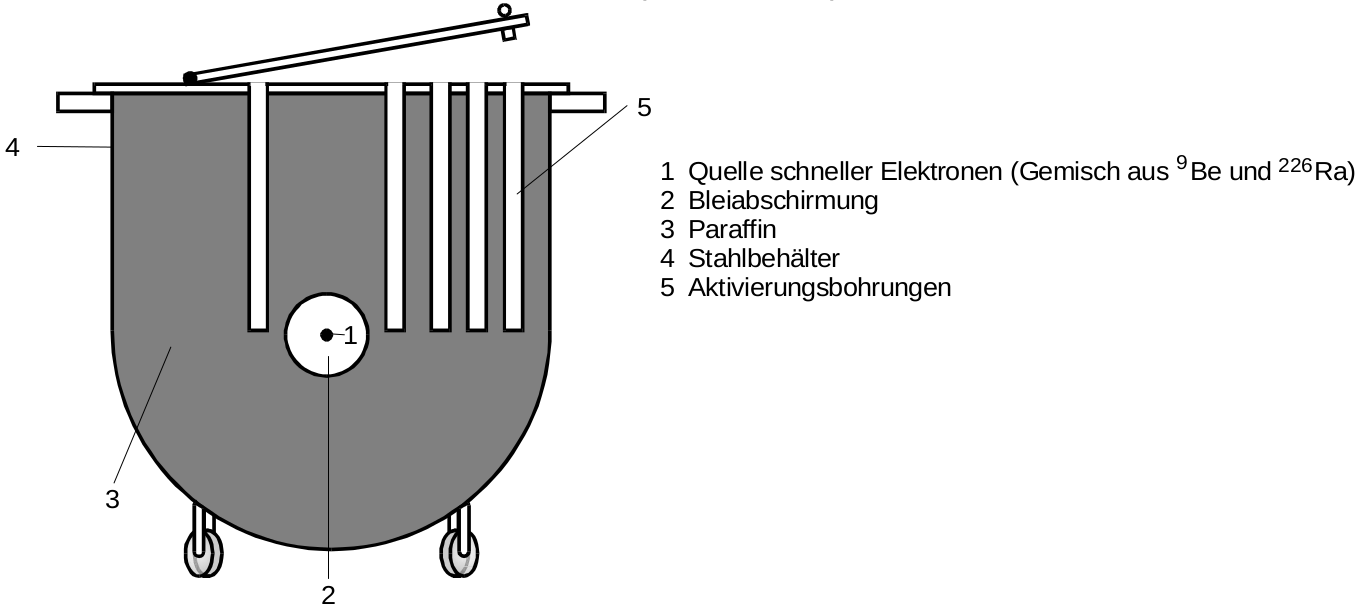
\includegraphics{content/toepfchen.png}
%	\label{fig:kochen}
%\end{figure}
%
Der Versuchsaufbau -- wie in Abbildung \ref{fig:aufbau} dargestellt -- besteht im Wesentlichen 
aus einem zerfallenden radioaktiven Isotop und einem Geiger-Müller-Zählrohr, welches die 
zerfallenden Kerne misst.
Das Geiger-Müller-Zählrohr ist entspricht einer mit Gas gefüllten Röhre. Trifft ein $\beta$-
oder $\gamma$- Teilchen auf ein Gasteilchen wird dieses ionisiert und kann aufgrund einer
anliegenden Spannung an der Röhre gemessen werden.
Dabei werden die gemessenen Zerfälle pro Messzeitintervall, welches am Zeitgeber einstellbar 
ist, an den Zählern 1 und 2 angezeigt. Nach jedem Messvorgang wird der Zähler umgeschaltet und 
der vorherige Wert auf dem aktuellen Zähler wird überschrieben. Der Versuchsaufbau ist mit
einer Blei-Abschirmung ausgestattet um die radioaktive Strahlung abzuschirmen.

Zur Erzeugung der radioaktiven Isotope wird das Objekt in Abbildung \ref{fig:kochen} verwendet.
Hierbei werden stabile Kerne mit niederenergetischen Neutronen beschossen. 
Da die Neutronen ihre Energie durch elastische Stöße an die Kerne übergeben und die maximale
Energie bei gleichen Massen der Stoßpartner erreicht wird, werden die Neutronen in einem 
Paraffinmantel gebremst, bis sie die optimale Energie besitzen.


\subsection{Versuchsbeschreibung}
\label{sec:Versuchsbeschreibung}
Zuerst soll die Strömungsgeschwindigkeit in Abhängigkeit des Doppler-Winkels bestimmt werden.
Hierfür wird am Ultraschallgenerator das SAMPLE VOLUME auf LARGE gestellt. 
Für die drei Teilrohre mit verschiedenem Durchmesser wird jeweils für die drei
Doppler-Winkel die Frequenzverschiebung $\Delta \nu$ mit der Ultraschallsonde gemessen.
Die Frequenzverschiebung kann am Rechner abgelesen werden.
Diese Messung wird für fünf verschiedene Geschwindigkeiten -- also fünf verschiedene 
Pumpleistungen $P$ der Zentrifugalpumpe -- wiederholt.

Weiterhin wird das Strömungsprofil des Rohrs mit einem Innendurchmesser von
$\SI{10}{\milli\meter}$ mit einem Doppler-Winkel von $\SI{15}{\degree}$ bei
maximaler Pumpleistung ($\SI{70}{\percent}$) erstellt.
Dafür muss am Ultraschallgenerator das SAMPLE VOLUME auf SIMPLE gestellt werden.
Die Messtiefe kann mit dem DEPTH-Regler variiert werden. Sie ist in $\si{\micro\second}$ 
angegeben. Der Umrechnungsfaktor in Acryl beträgt 
$\SI{1}{\micro\second}=\SI{5/2}{\milli\meter}$; in der Dopplerflüssigkeit hingegen
$\SI{1}{\micro\second}=\SI{3/2}{\milli\meter}$.
Gestartet wird die Messung bei einer Eindringtiefe kurz vor der Dopplerflüssigkeit -- bei
$\SI{13}{\micro\second}$ -- und diese wird dann in $\SI{0,5}{\micro\second}$-Schritten
bis zu einer Eindringtiefe von $\SI{19,5}{\micro\second}$ hochgeregelt.
Bei jedem Schritt wird die Frequenzverschiebung $\Delta \nu$ und der Streuintensitätswert 
am Rechner abgelesen.
Die Messung wird für eine Pumpleistung von $P=\SI{40}{\percent}$ wiederholt.
